\section*{Task 7}

\begin{figure}[H]
\centering
\begin{circuitikz}[american voltages]

    \node[circle, fill=black, inner sep=0pt] (TL) at (-3, 3) {};
    \node[circle, fill=black, inner sep=0pt] (TM) at (0, 3) {};
    \node[circle, fill=black, inner sep=0pt] (TR) at (3, 3) {};

    \node[circle, fill=black, inner sep=0pt] (MM) at (0, 0) {};
    \node[circle, fill=black, inner sep=0pt] (MR) at (3, 0) {};

    \node[circle, fill=black, inner sep=0pt] (BL) at (-3, -3) {};
    \node[circle, fill=black, inner sep=0pt] (BM) at (0, -3) {};
    \node[circle, fill=black, inner sep=0pt] (BR) at (3, -3) {};


    \draw (BL) to[vsourcesin, l=$U_{in}$] (TL);
    \draw (TL) -- (TR);
    \draw (BL) -- (BR);
    \draw (MM) to[zzD, l=$Z_1$, a=$6.8V$] (TM);
    \draw (BR) to[zzD, a=$4.7$, l=$Z_2$] (MR);
    \draw (TR) to[R, a=$R_2$, l=$3.3k\Omega$] (MR);
    \draw (MM) to[R, a=$R_1$, l=$10k\Omega$] (BM);
    \node[right] at (MM) {$A$};
    \node[left] at (MR) {$B$};
    \draw (BM) node[ground]{};

\end{circuitikz}
\caption{Current direction in negative cycle}
\end{figure}

\noindent
The voltage potential at node B is the same as the input until $Z_2$ opens at $V_B = 4.7V$. For $V_{in} < 0.7$, we have $V_A = 0V$ and $V_B = V_{in}$. For $V_in > 4.7V$, node B will remain at the same voltage since theres only the zenor voltage seperating it from ground. Node A is here also just ground voltage. When $V_{in} > 6.8$, the $Z_1$ diode will turn on and the voltage potential at node A is then $6.8V$ lower than the input. Important values for graphing will be the lowest and locally highest possible $V_{AB}$. the lowest possible is when no diode or just $Z_1$ is turned on, since then $V_A = 0V$. The locally highest value is when the input is at its highest.
\[
V_{AB\uparrow} = \left(10V-6.8V\right) - 4.7V = -1.5V
\]

\begin{figure}[H]
\centering
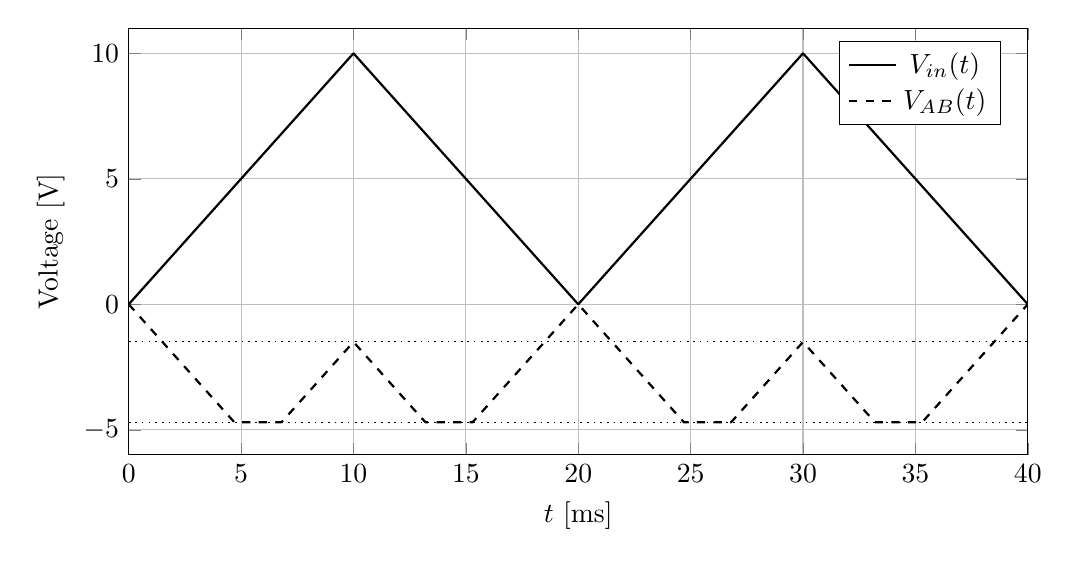
\begin{tikzpicture}
\begin{axis}[
    width=13cm,
    height=7cm,
    xlabel={$t$ [ms]},
    ylabel={Voltage [V]},
    xmin=0, xmax=40,
    ymin=-6, ymax=11,
    grid=both,
    legend pos=north east,
    domain=0:40,
    samples=1000
]

% Positive triangle wave: 0 -> 10 -> 0, period 20 ms
\addplot[thick]
{10 - abs(mod(x,20) - 10)};
\addlegendentry{$V_{in}(t)$}

% V_AB
\addplot[thick, dashed]
{
    % shorthand idea: u = 10 - abs(mod(x,20)-10)
    (10 - abs(mod(x,20)-10) <= 4.7) * (-(10 - abs(mod(x,20)-10)))
    +
    and(10 - abs(mod(x,20)-10) > 4.7,
        10 - abs(mod(x,20)-10) <= 6.8)
    * (-4.7)
    +
    (10 - abs(mod(x,20)-10) > 6.8)
    * ((10 - abs(mod(x,20)-10)) - 11.5)
};
\addlegendentry{$V_{AB}(t)$}

% Reference lines
\addplot[dotted] {-4.7};
\addplot[dotted] {-1.5};

\end{axis}
\end{tikzpicture}
\caption{Two periods of $V_{in}(t)$ and $V_{AB}(t)$.}
\label{fig:vab_two_periods}
\end{figure}